\documentclass{article}
\usepackage[utf8]{inputenc}
\usepackage[margin=2cm]{geometry}
%\usepackage{enumitem}
\usepackage{csquotes}

% maths packages
\usepackage{amsmath}
\usepackage{amssymb}
\usepackage{amsthm}
\usepackage{braket}

% remove space between ket and bra
\renewcommand\bra[1]{{\langle{#1}|}}
\makeatletter
\renewcommand\ket[1]{
  \@ifnextchar\bra{\k@t{#1}\!}{\k@t{#1}}
}
\renewcommand\ket[1]{
  \@ifnextchar\braket{\k@t{#1}\!}{\k@t{#1}}
}
\newcommand\k@t[1]{{|{#1}\rangle}}
\makeatother

% graphics packages
\usepackage{graphicx}
\usepackage{subcaption}
\usepackage[font={small,it}]{caption}
\usepackage{tikz}
\usetikzlibrary{positioning, circuits.logic.US}

% tikz ellipse arcs
\tikzset{
    partial ellipse/.style args={#1:#2:#3}{
        insert path={+ (#1:#3) arc (#1:#2:#3)}
    }
}

\title{QBF lit review?}
\author{Suzie Brown}
\date{\today}

% bibliography
\usepackage[round, sort&compress]{natbib}
\usepackage{har2nat} %%% Harvard reference style
\bibliographystyle{agsm}

% theorems
\newtheorem{thm}{Theorem}
\theoremstyle{definition}
\newtheorem{defn}{Definition}
\newtheorem{example}{Example}

% probability symbols
\newcommand{\PR}{\mathbb{P}}
\newcommand{\E}{\mathbb{E}}
\newcommand{\V}{\operatorname{Var}}
\newcommand{\iidsim}{\overset{iid}{\sim}}
\newcommand{\eqdist}{\overset{d}{=}}

% distributions
\newcommand{\Bern}{\operatorname{Bernoulli}}
\newcommand{\Geom}{\operatorname{Geom}}

% project-specific commands
\newcommand{\A}{\mathcal{A}}
\newcommand{\AND}{{\footnotesize AND }}
\newcommand{\NAND}{{\footnotesize NAND }}
\newcommand{\OR}{{\footnotesize OR }}
\newcommand{\NOR}{{\footnotesize NOR }}
\newcommand{\NOT}{{\footnotesize NOT }}

\begin{document}
%\maketitle

\section{Quantum information}
From the course by Noah Linden (University of Bristol) and discussion with Thomas Hebdige and David Jennings (Imperial College London). For a comprehensive introduction see for example \citet{nielsen2002} or \citet{wilde2013}.\\

Quantum mechanics is essentially linear algebra in a Hilbert space, with a few additional properties. The definitions in Sections \ref{sec:hilbert_defn} to \ref{sec:linear_ops} are exactly what you would find in a linear algebra course, apart from the notation.

\subsection{Dirac notation}
Dirac notation is a convenient way of denoting vectors such that it is easy to visually identify inner and outer products, and thus quickly recognise scalars, vectors and matrices:

\begin{itemize}
\item $\ket{v}$ denotes a column vector
\item $\bra{v}$ denotes a row vector
\item $\braket{u|v}$ denotes an inner product (resulting in a scalar)
\item $\ket{u}\bra{v}$ denotes an outer product (resulting in a matrix)
\end{itemize}
Additionally, $\overline{\alpha}$ denotes the complex conjugate of a scalar $\alpha$, and $U^\dag$ denotes the adjoint (conjugate transpose) of an operator $U$.

\subsection{Hilbert space}\label{sec:hilbert_defn}
A \emph{Hilbert space} is a vector space with an inner product $\braket{\cdot|\cdot}$ satisfying the following:
\begin{itemize}
\item $\bra{u} (\alpha\ket{v} + \beta\ket{w}) = \alpha\braket{u|v} + \beta\braket{u|w}$
\item $\braket{u|v} = \overline{\braket{v|u}}$
\item $\braket{v|v} \geq 0$ with equality iff $\ket{v}$ is the zero vector.
\end{itemize}

\subsection{Orthonormal bases}\label{sec:onb}
An \emph{orthonormal basis} of a Hilbert space $\mathcal{H}$ is a set of vectors $\{v_1,\dots,v_n\}$ in $\mathcal{H}$ such that:
\begin{itemize}
\item $\operatorname{span}(\{v_1,\dots,v_n\}) = \mathcal{H}$
\item $\braket{v_i|v_j} = \delta_{ij}$
\end{itemize}
Restricting to the space $\mathbb{C}^2$, which is all that is needed to understand the quantum Bernoulli factory, we have the \emph{computational basis} $\{\ket{0}, \ket{1}\} = \{(1,0)^T,(0,1)^T\}$. This is the canonical basis and is henceforth used wherever not specified otherwise. Since it is an orthonormal basis, every vector $\ket{v}$ in $\mathbb{C}^2$ has a unique representation
\begin{equation*}
\ket{v} = \alpha \ket{0} + \beta \ket{1} \equiv (\alpha,\beta)^T
\end{equation*}
for some $\alpha, \beta \in \mathbb{C}$. For reasons which will probably not become apparent in this treatment, we will restrict to \emph{normalised} vectors, requiring also $|\alpha|^2 + |\beta|^2 = 1$.
We will also consider two vectors equivalent if they differ only by an overall phase, i.e.\ $\ket{u} \equiv \ket{v}$ if $\ket{u} = e^{i\theta}\ket{v}$ for some $\theta$. This is because it is impossible to distinguish between two such vectors with any measurement.

To ensure coherency with the properties of the inner product, we have that
\begin{equation*}
\bra{v} = \overline{\alpha} \bra{0} + \overline{\beta} \bra{1}.
\end{equation*}
The inner product of $\ket{u} = u_0\ket{0} + u_1\ket{1}$ with $\ket{v} = v_0\ket{0} + v_1\ket{1}$ is therefore computed as
\begin{align*}
\braket{u|v} &= (\overline{u_0}\bra{0} + \overline{u_1}\bra{1}) (v_0\ket{0} + v_1\ket{1})\\
&= \overline{u_0}v_0\braket{0|0} + \overline{u_0}v_1\braket{0|1} + \overline{u_1}v_0\braket{1|0} + \overline{u_1}v_1\braket{1|1} \\
&= \overline{u_0}v_0 + \overline{u_1}v_1.
\end{align*}
One alternative choice of orthonormal basis which is worth mentioning is given by $\{\ket{+},\ket{-}\}$, consisting of the states
\begin{align*}
&\ket{+} := \frac{1}{\sqrt{2}}(\ket{0} + \ket{1}) \\
&\ket{-} := \frac{1}{\sqrt{2}}(\ket{0} - \ket{1}).
\end{align*}

\subsection{Linear operators}\label{sec:linear_ops}
A linear operator is an operator with the property
\begin{equation*}
A(\alpha\ket{u} + \beta\ket{v}) = \alpha A\ket{u} + \beta A\ket{v}.
\end{equation*}
It is therefore fully defined according to its action on an orthonormal basis. For instance, the quantum \NOT operator (usually denoted $X$) is defined by
\begin{align*}
& X\ket{0} = \ket{1} \\
& X\ket{1} = \ket{0}
\end{align*}
Equivalently, $X$ can be expressed as a matrix with respect to the computational basis:
\begin{equation*}
X = \left(\begin{matrix}
0 & 1 \\ 1 & 0
\end{matrix}\right)
\end{equation*}
In Dirac notation, X can be written in terms of outer products of basis states:
\begin{equation*}
X = \ket{0}\bra{1} + \ket{1}\bra{0}
\end{equation*}
Then if X acts on the state $\ket{v} = \alpha \ket{0} + \beta \ket{1}$, we have
\begin{align*}
X\ket{v} &= (\ket{0}\bra{1} + \ket{1}\bra{0})(\alpha \ket{0} + \beta \ket{1})\\
&= \alpha \ket{0}\braket{1|0} + \alpha \ket{1}\braket{0|0} + \beta \ket{0}\braket{1|1} +
\beta \ket{1}\braket{0|1}\\
&= \alpha \ket{1} + \beta \ket{0}
\end{align*}
as desired.

\begin{itemize}
\item A linear operator $U$ is said to be \emph{self-adjoint} (or \emph{hermitian}) if $U^\dag = U$
\item A linear operator $U$ is said to be \emph{unitary} if $UU^\dag = U^\dag U = I$
\end{itemize}
For example, the operator $X$ is self-adjoint and unitary. Crucially, untiary operators preserve normalisation, so they map states to states. It is also easy to see that unitary transformations are always reversible (i.e.\ the inverse operator exists).

\subsection{Rules of Quantum Mechanics}
\begin{enumerate}
\item \emph{States} of a quantum mechanical system correspond to normalised vectors in Hilbert space, up to an overall phase.
\item \emph{Evolutions} of the system correspond to unitary operators.
\item \emph{Measurements} on quantum states correspond to self-adjoint operators --- see below.
\end{enumerate}

\subsubsection{Spectral theorem and measurement}\label{sec:quantum_mmt}
The outcome of a measurement depends on the state of the system and the type of measurement performed.
The spectral theorem states that every self-adjoint operator $A$ can be represented by its spectral decomposition
\begin{equation}\label{eq:operator_diag}
A = \sum_{i} \lambda_i P_i
\end{equation}
where $\{\lambda_1,\dots, \lambda_k\}$ is the set of \emph{distinct} eigenvalues of $A$, and $P_i$ is the projection operator onto the eigenspace corresponding to eigenvalue $\lambda_i$.

When we measure a state $\ket{x}$ using operator $A$, the measurement outcome we observe is one of the eigenvalues of $A$. In particular, we observe $\lambda_i$ with probability $\bra{x} P_i \ket{x}$.
Making a measurement causes the system to collapse into the eigenstate corresponding to the observed eigenvalue; that is, the state after measurement is proportional to $P_i \ket{x}$.\\

\begin{example}\label{ex:quantum_mmt}
To give a concrete example, let us consider again the operator $X$. This operator has eigenvalues $\pm 1$ corresponding to eigenvectors (known as \emph{eigenstates} in quantum mechanics) $\ket{+}$ and $\ket{-}$ respectively.
Therefore $X$ admits the diagonal representation
\begin{equation*}
X= \ket{+}\bra{+} - \ket{-}\bra{-}
\end{equation*}
which is of the form \eqref{eq:operator_diag}.
Now suppose we make a measurement on the state $\ket{v} = \ket{0}$, using $X$.
The outcome of the measurement will be an eigenvalue of $X$: either $+1$ or $-1$. We observe the outcome $+1$ with probability
\begin{equation*}
\bra{v} P_{+1} \ket{v} = \braket{0|+}\braket{+|0} = 1/2
\end{equation*}
in which case the state after measurement is
\begin{equation*}
P_{+1} \ket{v} = \ket{+} \braket{+|0} \propto \ket{+}.
\end{equation*}
Alternatively, with probability 1/2 we observe the outcome $-1$ and the state after measurement is $\ket{-}$.
\end{example}

In this example, the two outcomes are equally likely because the state is `equidistant' from the two eigenstates of $X$. In general, outcomes that leave the state after measurement closer to the original state are more likely. We will see what is meant by distance between states in Section \ref{sec:bloch_sphere}.

A particularly important type of measurement is measurement in the computational basis. In this case the self-adjoint operator used is $0\cdot \ket{0}\bra{0} +1\cdot \ket{1}\bra{1} = \ket{1}\bra{1}$.
Measuring a state $\ket{v}=\alpha\ket{0} + \beta\ket{1}$ in the computational basis returns 0 with probability $|\alpha|^2$ or 1 with probability $|\beta|^2$. This is particularly useful in quantum computing algorithms because it deterministically converts the basis states $\ket{0}$ and $\ket{1}$ to their classical equivalents 0 and 1, ready for classical output.

\begin{figure}
\centering
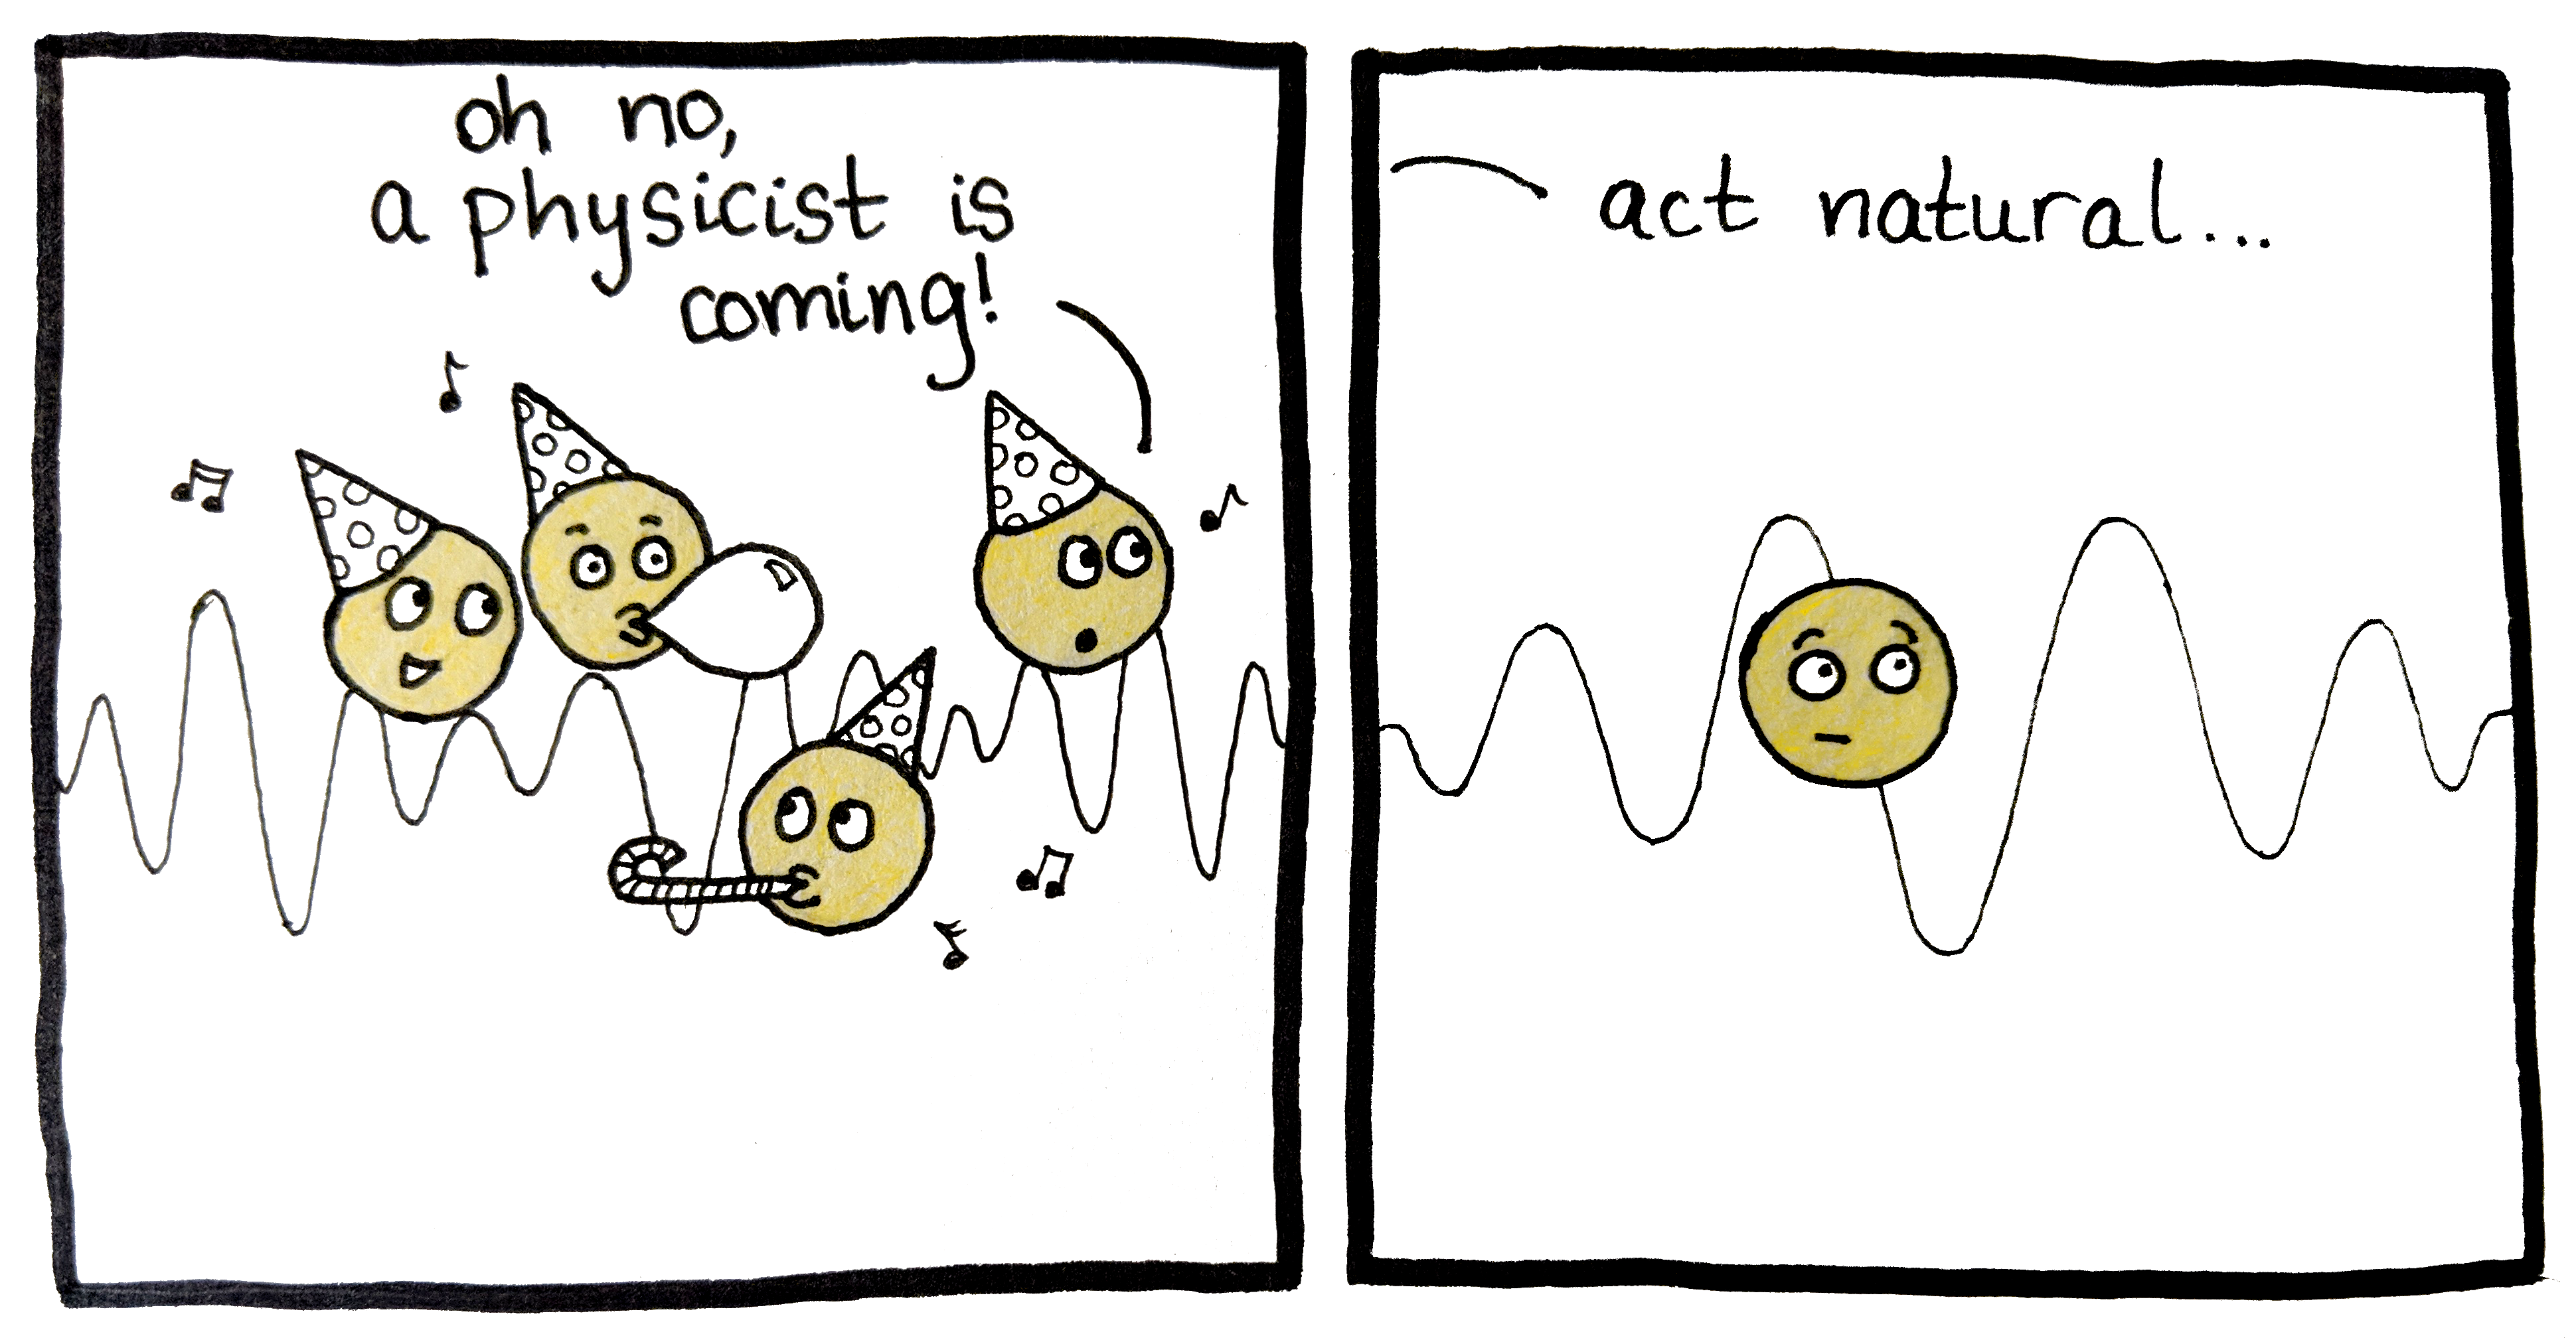
\includegraphics[width=0.8\textwidth]{qit_comic.png}
\caption{When a quantum system is in a superposition of states, making a measurement causes the system to collapse into the eigenstate corresponding to the observed eigenvalue.}
\label{fig:quantum_mmt_comic}
\end{figure}

\subsection{Quantum randomness}
It is worth remarking at this point on the difference between quantum and classical randomness.
As statisticians we are used to dealing with randomness, but we accept that randomness is always part of a model, and is not purported to exist in nature. We artificially introduce random variables into our models to account for a lack of information, either about the state of the system or about the (presumably deterministic) processes that govern certain phenomena.

On the contrary, our uncertainty about the outcome of a measurement on a quantum system is of a different kind. This uncertainty is not a symptom of our lack of knowledge: even when we know exactly the state of the system, as in Example \ref{ex:quantum_mmt}, we are still unable to predict with certainty the outcome of a measurement on the system. The randomness here is intrinsic; it really does exist in nature.

\subsection{Pure and mixed states}
So far we have only encountered \emph{pure states}, like $\ket{0}$ or $\ket{+}$. But we can also consider probabilistic mixtures of pure states, known as \emph{mixed states}, like
\begin{equation*}
\ket{v} = \sum_{i} p_i \ket{v_i}
\end{equation*}
where $\{p_i\}$ is a probability distribution and the $\ket{v_i}$ are pure states.
You can think of this as a `source' which emits a state $\ket{v_i}$ with probability $p_i$.
A classical analogue is a bit which takes the value 1 with probability $p$ or 0 with probability $1-p$ (a $p$-coin). In this case, we can say that the expected value of the bit is $p$.

There is no full ordering on the set of quantum states, so it is not possible to define the expected value of a mixed state. However, we can calculate the expected value of a measurement on a mixed state, using the state's \emph{density operator}.

\subsubsection{Density operators}
The density operator of a mixed state $\ket{v} = \sum_{i} p_i \ket{v_i}$ is given by
\begin{equation*}
\rho = \sum_{i} p_i \ket{v_i}\bra{v_i}.
\end{equation*}
Different mixtures of states may have the same density operator, but in this case is is impossible to distinguish between them by any measurement. For example, a source which emits $\ket{0}$ or $\ket{1}$ each with probability 1/2 has the same density operator $\rho = I/2$ as a source which emits $\ket{+}$ or $\ket{-}$ each with probability 1/2, and the two sources are indistinguishable.

Suppose we measure a mixed state using the self-adjoint operator $A= \sum_k \lambda_k P_k$, where $\{\lambda_k\}$ are the distinct eigenvalues of $A$ and $P_k$ the projection onto the corresponding eigenspace. Recall (from Section \ref{sec:quantum_mmt}) that the outcome of the measurement will be an eigenvalue of $A$. The probability of observing a particular outcome is
\begin{equation*}
\PR(\text{observe }\lambda_j) = \sum_i p_i \bra{v_i} P_j \ket{v_i} = tr(\rho P_j)
\end{equation*}
where $tr(\cdot)$ denotes the trace of an operator.
Note that $tr(\rho)=1$ because the states are normalised and $\{p_i\}$ is a probability distribution.

The state $\rho = I/2$ is called the \emph{maximally mixed} state; it expresses complete ignorance, like a classical (1/2)-coin.

\subsection{The Bloch sphere}\label{sec:bloch_sphere}
Density operators have a neat geometrical representation as points in a unit sphere (Figure \ref{fig:qubit_state_space}). This is called the \emph{Bloch sphere}, and can be thought of as the state space of a quantum bit (qubit).

An arbitrary pure state can be written in the form
\begin{equation*}
\ket{v} = e^{i\psi} \left[ \cos \left(\frac{\theta}{2}\right) \ket{0} + e^{i\phi} \sin \left(\frac{\theta}{2}\right) \ket{1} \right].
\end{equation*}
Since the overall phase $e^{i\psi}$ can be ignored, the state is parametrised by two angles $\theta$ and $\phi$. Taking these as spherical coordinates with unit radius, we can think of each pure state as a point on the unit sphere (or equivalently, a unit vector). Orthogonal states lie opposite each other on the Bloch sphere.
% if theta=0, phi doesn't have any effect...? -use proper coordinates for dens oper

Mixed states can also be represented in the Bloch sphere. The Bloch vector for a mixed state is found by taking the weighted average of the Bloch vectors of its component pure states. Due to the triangle inequality, mixed states therefore lie strictly inside the unit sphere.
This illustrates that several different mixtures of states can have the same density operator. Qubit states are distinguishable if and only if they correspond to different points in the Bloch sphere. %really iff?
The notion of `distance' between states is formalised as Euclidean distance between points in the Bloch sphere: orthogonal states are the `most different' and lie the furthest possible distance apart on the sphere; while the maximally mixed state is at the centre of the sphere, equidistant from every pure state.

There is an analogy here with classical information. The state space of a classical bit is the unit interval: its value could be 0 or 1, or we could take a probabilistic mixture of the two. The `pure' states then are 0 and 1, which lie on the `surface' of the interval, while `mixed' states lie strictly inside the interval (Figure \ref{fig:cbit_state_space}). 


Finally, unitary operators are rotations of the Bloch sphere. This illustrates that unitary transformations are reversible.

\begin{figure}
\centering
\begin{subfigure}{0.25\linewidth}
\centering
\begin{tikzpicture}
\draw (0,4) -- (0,-4);
\filldraw (0,4) circle (2pt) node[anchor=south] {0};
\filldraw (0,-4) circle (2pt) node[anchor=north] {1};
\end{tikzpicture}
\caption{Classical bit}
\label{fig:cbit_state_space}
\end{subfigure}%
\begin{subfigure}{0.75\linewidth}
\centering
\begin{tikzpicture}
\draw (0,0) circle (4cm);
\draw (0,4) -- (0,-4);
\draw[gray] (-4,0) -- (4,0);
\draw[gray] (0,0) ellipse (4cm and 1.5cm);
\filldraw (0,4) circle (2pt) node[anchor=south] {$\ket{0}\bra{0}$};
\filldraw (0,-4) circle (2pt) node[anchor=north] {$\ket{1}\bra{1}$};
\filldraw (-4,0) circle (2pt) node[anchor=east] {$\ket{+}\bra{+}$};
\filldraw (4,0) circle (2pt) node[anchor=west] {$\ket{-}\bra{-}$};
%\filldraw (0,0) circle (2pt) node [anchor=west] {$I/2$};
\draw[ultra thick, ->] (0,0) -- (2,2);
\draw[dotted] (0,0) -- (2,-0.5);
\draw[dotted] (2,-0.5) -- (2,2);
%
\draw[blue] (0,0.5) arc (90:45:0.5);
\draw[red] (0,0) [partial ellipse=180:332:0.5cm and 0.25cm];
\node[red] at (-0.4,-0.4) {$\phi$};
\node[blue] at (0.3, 0.7) {$\theta$};
\end{tikzpicture}
\caption{Qubit}
\label{fig:qubit_state_space}
\end{subfigure}

\caption{State space of classical bits versus qubits. The state space of a classical bit is the line segment $[0,1]$. The `pure' states 0 and 1 are at the endpoints, and probabilistic mixtures of the two lie inbetween. The state space of a qubit is the Bloch sphere. Pure states are on the surface of the sphere, and mixed states are in the interior. The centre of the sphere is the maximally mixed state $\rho=I/2$.}
\end{figure}
% where should theta & phi actually be measured from? - values at 0,+ etc.

\bibliography{qbf.bib}
\end{document}